\documentclass[a4paper,12pt]{report}

\usepackage{color}
\usepackage{mathtools}
\usepackage[brazilian]{babel}
\usepackage[utf8]{inputenc}
\usepackage[T1]{fontenc}
\usepackage{tikz}
\usetikzlibrary{arrows.meta}
\usetikzlibrary{automata,positioning}
\usepackage{pgfplots}
\usepackage{filecontents}
\usepackage{cancel}
\usetikzlibrary{arrows.meta}
\usetikzlibrary{arrows.meta}
\usepackage{bm}
\usepackage{mathrsfs}
\usepackage{blkarray}
\usepackage{gensymb}
\usepackage{graphicx}
\graphicspath{/Users/gustavo/Desktop/Estatística\ Matemática}
\usepackage{amssymb}
\usepackage{tkz-euclide}
\usepackage[margin=0.1in]{geometry}
\usepackage{enumitem} 
\usepackage{accents}


\author{}
\geometry{textwidth=6in, textheight=9in, marginparsep=7pt, marginparwidth=.6in, top=30mm, bottom=25mm}

\title{Exercícios Inferência Matemática\\
Barry R. James - Probabilidade: um curso em nível intermediário\\
Capítulo 1 e Capítulo 2
}
\date{}
\begin{document}
	\maketitle
	\tableofcontents	
	\newpage
	
	
	\chapter{Páginas 26 - 32}
	\section{Questão 1}
	\begin{enumerate}[label=(\alph*)]
		\item  $\equiv (ii)$
		\item $\equiv (iii)$
		\item $\equiv (iv)$
		\item $\equiv (i)$
	\end{enumerate}


       \section{Questão 2}


$P\bigg(\bigcup\limits_{n=1}^{\infty}A_n \bigg) \le \sum\limits_{n=1}^{\infty}P(A_n)$\\
Se os subconjuntos $B_1,B_2,\ldots,B_n\subset B $ são disjuntos, então:\\
$P\bigg(\bigcup\limits_{n=1}^{\infty}B_n \bigg) = \sum\limits_{n=1}^{\infty}P(B_n) $ ($\sigma$-Aditividade)\\
Podemos construir $B$ de tal forma que:
$$B\subset A \Rightarrow P(B)\le  P(A)$$
Podemos também escrever os subconjuntos $A_n$ de tal forma que eles sejam disjuntos:
$$B_n = A_n - \bigcup\limits_{m=1}^{n-1}A_m\Rightarrow B_n\subset A_n, \ \ n>1 $$
$$\bigcup\limits_{n=1}^{\infty}B_n=\bigcup\limits_{n=1}^{\infty}A_n $$
$$ P\bigg(\bigcup\limits_{n=1}^{\infty}A_n\bigg) =P\bigg(\bigcup\limits_{n=1}^{\infty}B_n\bigg) = \sum\limits_{n=1}^{\infty} P(B_n)
\le \sum\limits_{n=1}^{\infty}P(A_n)
$$
$\therefore  $
$$P\bigg(\bigcup\limits_{n=1}^{\infty}A_n \bigg) \le \sum\limits_{n=1}^{\infty}P(A_n)$$
\newpage
\section{Questão 3}

		\begin{enumerate}[label=(\alph*)]
		\item
		Note que:
		$$\bigcap\limits_{i=1}^{\infty}A_i =\bigg(\bigcup\limits_{i=1}^{\infty}A_i^c\bigg)^c  $$
		Então:
				$$P\bigg(\bigcap\limits_{i=1}^{\infty}A_i\bigg) =P\bigg(\bigg(\bigcup\limits_{i=1}^{\infty}A_i^c\bigg)^c \bigg) 
				=
				1 - P\bigg(\bigcup\limits_{i=1}^{\infty}A_i^c\bigg)\ge 1- \sum\limits_{i=1}^{n} P(A_i^c)
				$$
				$$
				\Rightarrow P\bigg(\bigcap\limits_{i=1}^{\infty}A_i\bigg) \ge 1- P\bigg(\bigcup\limits_{i=1}^{\infty}A_i^c\bigg)
				$$
		
		\item 
		
		$$P(A_k)\ge 1-\varepsilon $$`
		$$\sum\limits_{k=1}^{n}P(A_k) \ge \sum\limits_{i=1}^{n}(1-\varepsilon)=n-n\varepsilon$$
		$$\sum\limits_{k=1}^{n} P(A_k)\ge P\bigg(\bigcup\limits_{k=1}^{n}A_k \bigg)  $$
			$$  \sum\limits_{k=1}^{n}P(A_k^c)\ge P\bigg(\bigcup\limits_{k=1}^{n}A_k \bigg)^c $$
		$$  n- \sum\limits_{k=1}^{n}P(A_k) \ge 1- P\bigg(\bigcap\limits_{n=1}^{n}A_k \bigg) $$
				$$  \sum\limits_{k=1}^{n}P(A_k) \le -1+n+ P\bigg(\bigcap\limits_{n=1}^{n}A_k\bigg) $$
								$$ n-n\varepsilon \le -1+n+ P\bigg(\bigcap\limits_{k=1}^{n}A_k \bigg) $$
									$$ 1-n\varepsilon \le P\bigg(\bigcap\limits_{k=1}^{n}A_k \bigg) $$
									\newpage
									\item 
									 
						 
						 $$P\bigg(\bigcap\limits_{k=1}^n A_k \bigg) \ge 1-\sum\limits_{k=1}^n P(A_k^c)$$
									Sabemos que 
									
									$$P\bigg(\bigcup\limits_{k=1}^{n}A_n \bigg) \le \sum\limits_{n=1}^{n}P(A_k)$$
									$$\Rightarrow P\bigg(\bigcup\limits_{n=1}^{n}A_n^c \bigg) \le \sum\limits_{n=1}^{n}P(A_n^c)$$
									$$\Rightarrow P\bigg(\bigcap\limits_{n=1}^{\infty}A_n \bigg)^c \le \sum\limits_{n=1}^{n}P(A_n^c) $$
									$$\Rightarrow 1-P\bigg(\bigcap\limits_{n=1}^{\infty}A_n \bigg) \le \sum\limits_{n=1}^{n}P(A_n^c)$$
								$$\Rightarrow P\bigg(\bigcap\limits_{n=1}^{\infty}A_n \bigg) \ge1- \sum\limits_{n=1}^{\infty}P(A_n^c)$$
		\end{enumerate}
		
		
		\section{Questão 4}
		\begin{enumerate}[label=\alph*)]
			\item 
	
		$$P(A_n)=0 $$
		Sabemos que:
		$$P\bigg(\bigcup\limits_{n=1}^{\infty}A_n \bigg) \le \sum\limits_{n=1}^{\infty}P(A_n)=0$$
		Note que por hipótese $\bigcup\limits_{n=1}^{n}A_n  \ge 0 $ pois se tratam de eventos aleatórios de $\Omega$. Então:
		$$ 0\ge P\bigg(\bigcup\limits_{n=1}^{n}A_n \bigg) \le 0 \Rightarrow  P\bigg(\bigcup\limits_{n=1}^{n}A_n \bigg) =0$$
		\item 
		$$P\bigg(\bigcap\limits_{n=1}^{\infty}A_n \bigg) = 1- P\bigg(\bigcup\limits_{n=1}^{\infty}A_n^c  \bigg) \ \ \ \ \ (*) $$
		Note que pelo teorema anterior:
		
		$$1- P\bigg(\bigcup\limits_{n=1}^{\infty}A_n^c  \bigg)\le 1- \sum\limits_{n=1}^{\infty}P(A_n^c) 
		=
		1- \sum\limits_{n=1}^{\infty}(1-P(A_n))= 1- \sum\limits_{n=1}^{\infty}(1-1)=1 
		$$
		$$\therefore 1- P\bigg(\bigcup\limits_{n=1}^{\infty}A_n^c  \bigg)\le1 \underset{(*)}{\Rightarrow}  P\bigg(\bigcap\limits_{n=1}^{\infty}A_n  \bigg)\ge 1$$
		Porém essa expressão é limitada superiormente pois $\bigcap\limits_{n=1}^{\infty}A_n\subset \Omega $ e $P\bigg(\bigcap\limits_{n=1}^{\infty}A_n\bigg)\le \Omega =1$\\
		Logo: 
		$$ 1\ge P\bigg(\bigcap\limits_{n=1}^{\infty}A_n  \bigg)\le 1$$
		$$\therefore P\bigg(\bigcap\limits_{n=1}^{\infty}A_n  \bigg)=1$$
			\end{enumerate}

		
		\section{Questão 5}
		É fácil ver  que  $P(A_n){\longrightarrow}1 \Leftrightarrow A_n = \Omega $. Além disso, sabemos que  $P(B\cap\Omega)= B, \forall  B\subseteq \Omega$.\\
		Então, $P(A_n\cap B_n)\rightarrow p$ quando $B_n \rightarrow p $
		
	
		\section{Questão 6}
		\begin{enumerate}[label=\alph*)]
			\item
			Para provarmos que $\mathscr A \cap \mathscr B$  é  $\sigma$-algebra de $\Omega$, basta mostrar que essa intersecção satisfaz as 3 propriedades de uma $\sigma$-algebra.\\
			\begin{itemize}
				\item  $\mathscr A \cap \mathscr B\ne \emptyset $ pois  por definição $\mathscr A$ e $\mathscr B$ são não vazios.
				
				\item ($\mathscr A \cap \mathscr B)^c$ =$\mathscr A^c \cup \mathscr B^c$. Por hipótese, $\mathscr A^c $ e $ \mathscr B^c$ pertencem ao subconjunto de partes de $\Omega$ e pela propriedade 3 a união desses dois elementos também pertence ao subconjunto de partes de $\Omega$.
				\item 
			\end{itemize}
			\item
		Sejam $A_n$ $\sigma$-algebras contendo $\mathscr{C}$. Entao $\bigcap\limits_{n=1}^\infty \mathscr{A}_n$ é uma $\sigma$-algebra minimal que contem $\mathscr{C}$.\\
		\\
		\underline{Sol}:\\
		\\
		Por hipotese, tem-se que:\\
		\\
		$\mathscr{A}_n, n=1,2,\ldots$, e $\sigma$-algebra contendo $\mathscr{C}$.\\
		\\
		Como  $\bigcap\limits_{n=1}^\infty \mathscr{A}_n \subset \mathscr{A}$ para algum n, entao  $\bigcap\limits_{n=1}^\infty \mathscr{A}_n$ contem $\mathscr{C}$. Entao basta mostrar que  $\bigcap\limits_{n=1}^\infty \mathscr{A}_n$ é $\sigma$-algebra.\\
		\\
		De fato:\\
		Temos que $\mathscr{C} \in \bigcap\limits_{n=1}^\infty \mathscr{A}_n$, então (i) e satisfeito.\\
		Por outro lado,\\
		(ii) Se $A \in \bigcap\limits_{n=1}^\infty \mathscr{A}_n$  entao $A\in \mathscr{A}_n, \forall n$. Sendo $\mathscr{A}_n$ $\sigma$-algebra, temos que:\\
		\\
		$A^c \in \mathscr{A}_n,\forall n$\\
		Dai, $A^c \in \bigcap\limits_{n=1}^\infty \mathscr{A}_n$ \\
		(iii) Sejam $A_1,A_2,\ldots$ eventos de $\bigcap\limits_{n=1}^\infty \mathscr{A}_n$ .\\
		Então $A_1,A_2,\ldots \in \mathscr{A}, \forall n=1,\ldots$\\
		Daí   $\bigcup\limits_{i=1}^\infty A_i\in \mathscr{A}_n, \forall n=1,2,\ldots$\\
		Assim,  $\bigcup\limits_{i=1}^\infty A_i\in \bigcap\limits_{n=1}^\infty \mathscr{A}_n$\\
		 \end{enumerate} 
		


	

	\section{Questão 7}
	
$$	\limsup\limits_{n\rightarrow \infty} A_n =\liminf\limits_{n\rightarrow \infty} A_n =A,A=\lim\limits_{n\rightarrow \infty} A_n $$
$$\Rightarrow \lim\limits_{n\rightarrow \infty}P(A_n)=P(A)  $$	

\underline{Seja}:
\begin{enumerate}[label=\alph*)]
	\item $\limsup\limits_{n\rightarrow \infty} A_n =A=\lim\limits_{n\rightarrow \infty} A_n  $\\
	Defina
	$$\limsup\limits_{n\rightarrow \infty} A_n = \bigcap\limits_{n=1}^\infty \bigg( \underbrace{\bigcup\limits_{i=n}^{\infty}}_{B_n}\bigg) $$
	$$B_1\supset B_2 \ldots \supset B_n \supset \ldots \supset \bigcap\limits_{i=1}^{\infty}B_n= \bigcap\limits_{n=1}^\infty\bigg(\bigcup\limits_{i=n}^\infty A_i\bigg)=\limsup\limits_{n\rightarrow \infty} A_n=A,$$
	
	Então, pela continuidade da probabilidade, tem-se que:
	
	$$\displaystyle{\lim_{n \to \infty}}  P(B_n)=P(A) $$
	ou 
		$$\displaystyle{\lim_{n \to \infty}}  P\bigg(\bigcup\limits_{i=n}^\infty A_i\bigg)=P(A) \ \ \ \ \ \ (1)$$
		Por outro lado,
		$$A_n \subset  \bigcup\limits_{i=n}^\infty A_i$$
		Assim, 
		$$P(A_n)\le  P\bigg(\bigcup\limits_{i=n}^\infty A_i \bigg)$$
		e 
		$$\displaystyle{\lim_{n \to \infty}} P(A_n)\le \displaystyle{\lim_{n \to \infty}} P\bigg(\bigcup\limits_{i=n}^\infty A_i \bigg) \overset{(1)}{=} P(A)  $$
		$$\therefore \displaystyle{\lim_{n \to \infty}} P(A_n)\le P(A) \ \ \ \ (2) $$
		
		\item Se $\liminf\limits_{n\rightarrow \infty} A_n = \displaystyle{\lim_{n \to \infty}} A_n=A,$\\
		Então 
		$$ \displaystyle{\lim_{n \to \infty}} A_n \ge P(A) \ \ \ \ \ \ \ \ (3)$$
		
		A prova está completa a partir de (2) e (3)
	
\end{enumerate}
\newpage
	\section{Questão  8}
$$\Omega: \bigg\{ \omega = d_1,d_2):d_1,d_2 \in \{1,2,3,4,5,6\} \bigg\} $$
Vitória 1 : $V_1=\bigg\{(d_1,d_2): d_1+d_2 \in \{7,11 \}  \bigg\} $\\
Derrota 1 : $D_1=\bigg\{(d_1,d_2): d_1+d_2 \in \{2,3,12 \}  \bigg\} $\\
Continuação: $C=\bigg\{4,5,6,8,9,10\bigg\} $\\
A partir daqui, a probabilidade de vitória está condicionada ao valor obtido em C, caso o jogador obtenha o mesmo resultado em dois lançamentos consecutivos ele ganha, caso contrário, ele perde. Note que o jogo continua até o jogador ganhar ou perder, podendo ter potencialmente um numero elevado de jogadas de dados, então, é interessante incorporamos o final do jogo na medida de probabilidade.\\
Podemos considerar que  a vitória se dá quando o jogador consegue atingir a condição de vitória antes da condição de derrota, que é probabilisticamente  análogo considerar que a foi alcançada a vitória ou a derrota.
\\
Utilizando o teorema de Bayes:
$$P\bigg(\{s=x\}|\{s=x\}\cup\{s=7\}\bigg)=\frac{P\bigg(\{s=x\}\cap \bigg\{\{s=x\}\cup\{s=7\} \bigg\}\bigg)}{P\bigg( \bigg\{ \{s=x \}\cup\{s=7\}\bigg\} \bigg)} $$
$$
\therefore
P\bigg(\{s=x\}|\{s=x\}\cup\{s=7\}\bigg)=
\frac{P\bigg(\{s=x\}\bigg)}{P\bigg( \bigg\{ \{s=x \}\cup\{s=7\}\bigg\} \bigg)} 
$$


Sendo assim, tomando $s=d_1+d_2$ o evento em que a soma dos números nas faces superiores dados leva a vitória, temos que a probabilidade de vitória dado que a $s\in C$ pode ser expressa por:\\
\\
 $\overbrace{P(\{s=4\})}^{\text{Primeiro lançamento}}\cdot P(\{s=7\}|\{s=4\} \cup \{s=7\}) )= \frac{3}{36}\cdot\frac{\frac{3}{36}}{\frac{9}{36}}=\frac{3}{36}\cdot\frac{3}{9}$\\
  $P(\{s=5\})\cdot P(\{s=5\}|\{s=5\} \cup \{s=7\}) = \frac{4}{36}\cdot\frac{\frac{4}{36}}{\frac{10}{36}}=\frac{4}{36}\cdot\frac{4}{10}$\\
   $P(\{s=6\})\cdot P(\{s=6\}|\{s=6\} \cup \{s=7\}) = \frac{5}{36}\cdot\frac{\frac{5}{36}}{\frac{11}{36}}=\frac{5}{36}\cdot\frac{5}{11}$\\
    $P(\{s=8\})\cdot P(\{s=8\}|\{s=8\} \cup \{s=7\}) = \frac{5}{36}\cdot\frac{\frac{5}{36}}{\frac{11}{36}}=\frac{5}{36}\cdot\frac{5}{11}$\\
     $P(\{s=9\})\cdot P(\{s=9\}|\{s=8\} \cup \{s=7\}) =\frac{4}{36}\cdot\frac{\frac{4}{36}}{\frac{10}{36}}=\frac{4}{36}\cdot\frac{4}{10}$\\
      $P(\{s=10\})\cdot P(\{s=10\}|\{s=10\} \cup \{s=7\}) = \frac{3}{36}\cdot\frac{\frac{3}{36}}{\frac{9}{36}}=\frac{3}{36}\cdot\frac{3}{9}$\\
      \\
Logo, a probabilidade de vitória é dada por:

$$P(\{G\})=\frac{8}{36}+2\bigg(\frac{3}{36}\cdot\frac{3}{9}+\frac{4}{36}\cdot\frac{4}{10} +\frac{5}{36}\cdot\frac{5}{11}\bigg)=0.4929293 $$
Analogamente, se considerarmos a probabilidade de derrota, temos:
$$
P\bigg(\{s=7\}|\{s=x\}\cup\{s=7\}\bigg)=
\frac{P\bigg(\{s=7\}\bigg)}{P\bigg( \bigg\{ \{s=x \}\cup\{s=7\}\bigg\} \bigg)} 
$$
endo assim, tomando $s=d_1+d_2$ o evento em que a soma dos números nas faces superiores dados leva a derrota, temos que a probabilidade de derrota dado que a $s\in C$ pode ser expressa por:\\
\\
$P(\{s=4\})\cdot P(\{s=7\}|\{s=4\} \cup \{s=7\}) = \frac{3}{36}\cdot\frac{\frac{6}{36}}{\frac{9}{36}}=\frac{3}{36}\cdot\frac{6}{9}$\\
$P(\{s=5\})\cdot P(\{s=7\}|\{s=5\} \cup \{s=7\}) = \frac{4}{36}\cdot\frac{\frac{6}{36}}{\frac{10}{36}}=\frac{4}{36}\cdot\frac{6}{10}$\\
$P(\{s=6\})\cdot P(\{s=7\}|\{s=6\} \cup \{s=7\}) = \frac{5}{36}\cdot\frac{\frac{6}{36}}{\frac{11}{36}}=\frac{5}{36}\cdot\frac{6}{11}$\\
$P(\{s=8\})\cdot P(\{s=7\}|\{s=8\} \cup \{s=7\}) = \frac{5}{36}\cdot\frac{\frac{6}{36}}{\frac{11}{36}}=\frac{5}{36}\cdot\frac{6}{11}$\\
$P(\{s=9\})\cdot P(\{s=7\}|\{s=8\} \cup \{s=7\}) =\frac{4}{36}\cdot\frac{\frac{6}{36}}{\frac{10}{36}}=\frac{4}{36}\cdot\frac{6}{10}$\\
$P(\{s=10\})\cdot P(\{s=7\}|\{s=10\} \cup \{s=7\}) = \frac{3}{36}\cdot\frac{\frac{6}{36}}{\frac{9}{36}}=\frac{3}{36}\cdot\frac{6}{9}$\\
\\
Logo, a probabilidade de derrota é dada por:

$$P(\{G\})=\frac{4}{36}+2\bigg(\frac{3}{36}\cdot\frac{6}{9}+\frac{4}{36}\cdot\frac{6}{10} +\frac{5}{36}\cdot\frac{6}{11}\bigg)=0.5146605 $$

\newpage

\section{Questão  9}
Podemos fixar $a$ sorvetes do sabor $A$ e $b$ sorvetes do sabor $B$ de acordo com as preferências, sendo assim, resta distribuir 
$(n-a)$ e $(n- b)$ sorvetes entre as $2n-a- b$ pessoas restantes, que são indiferentes ao sabor. Além disso, existem $ \binom{2n}{n}$ maneiras de distribuir os 2n entre os indivíduos.

Logo, a probabilidade do evento de interesse ocorrer é:
$$P(A) = \frac{\binom{2n-a- b}{n-a}}{\binom{2n}{n}} $$



\section{Questão  10}
Seja x o número de retiradas até obter uma carta de número par do conjunto de cartas enumeradas de 1 a 10, um modelo probabilístico possível é:
$$
P_X(x)= 
\begin{cases}
\frac{5}{10}, \ \ \ x=1\\
\frac{5}{10}\cdot\frac{5}{9}, \ \ \ x=2\\
\frac{5}{10}\cdot\frac{5}{9}\cdot\frac{5}{8}, \ \ \ x=3\\
\frac{5}{10}\cdot\frac{5}{9}\cdot\frac{5}{8}\cdot\frac{5}{7}, \ \ \ x=4\\
\frac{5}{10}\cdot\frac{5}{9}\cdot\frac{5}{8}\cdot\frac{5}{7}\cdot\frac{5}{6}, \ \ \ x=5\\
\frac{5}{10}\cdot\frac{5}{9}\cdot\frac{5}{8}\cdot\frac{5}{7}\cdot\frac{5}{6}\cdot\frac{5}{5}, \ \ \ x=6\\
\end{cases}
$$
=
$$
P_X(x)= 
\begin{cases}
\frac{1}{2}, \ \ \ \ x=1\\
\frac{5}{18}, \ \ \ \ x=2\\
\frac{5}{36}, \ \ \ \ x=3\\
\frac{5}{84}, \ \ \ \ x=4\\
\frac{5}{252},\ \ \ \ x=5\\
\frac{5}{1260},\ \ \ \ x=6\\
\end{cases}
$$
\newpage

\
\section{Questão  11}
\begin{enumerate}[label=\alph* )]
	\item $$\Omega=\bigg\{(x,y): x,y\in [0,1] \bigg\} $$
O espaço de probabilidade pode ser definido por:
$$(\Omega,\mathscr B^2,p_x) $$
Onde $\mathscr B^2$ é a sigma algebra de borel do quadrado definido em $\mathbb R^2$ e $p_x$ é a medida de probabilide de Lebesgue.
\item 
$$\Omega = \bigg\{\omega= \{r_1,r_2,\ldots \}:  r_i\in \{A1,A2,\ldots,K4 \},i=1,2\ldots,\bigg\}  $$
$$P(r=k)= \frac{4}{52}\bigg(\frac{48}{52}\bigg)^{k-1}, \ \ \ k=1,2,3,\ldots $$

\item 

$$\Omega = \bigg\{ (r_1,r_2,\ldots,r_15):  r_i\in \{p,p,p,p,p,p,p,p,p,v,v,v,v,v,b \},i=1,\ldots,15 \bigg\} $$
$$P(p,v,b)= \frac{15!}{p!\cdot v!\cdot b!} \bigg(\frac{9}{15}\bigg)^p\bigg(\frac{5}{15}\bigg)^v\bigg(\frac{1}{15}\bigg)^b $$
\item 
$$\Omega = \bigg\{ (r_1,r_2,\ldots,r_{15}):  r_i\in \{p,p,p,p,p,p,p,p,p,v,v,v,v,v,b \},i=1,\ldots,15 \bigg\} $$
$$P(p,v,b) =\frac{\binom{9}{p}\binom{5}{v}\binom{1}{b}}{\binom{15}{p+v+b}}= 1 $$
\end{enumerate}
\newpage
\section{Questão 12}
\begin{enumerate}[label=\alph*)]
	\item 
	$$
	P_X(k)=
	\frac{\binom{4}{k}\binom{48}{4-k} }{\binom{52}{4}}, \ \ k=0,1,2,3,4 $$
	\item 
	$$
	P_X(k)= \binom{4}{k} \bigg(\frac{4}{52}\bigg)^{k}\bigg( \frac{48}{52}\bigg)^{4-k}, \ \ \ k=0,1,2,3,4
	$$
	\item É fácil ver que é mais fácil obter 4 reis no caso com reposição pois a probabilidade de retirada do rei é sempre maior ou igual do que no caso sem reposição.
\end{enumerate}


\newpage
\section{Questão 13}
\begin{enumerate}[label=\alph*)]
	\item 

Sejam A ,B e C eventos de $\Omega$.\\
Podemos definir a união dos  eventos como, tomando $D=B\cup C$:
$$A\cup D= (A-D)\cup(A\cap D)\cup(D-A) $$
Aplicando probabilidade, temos:
$$P(A\cup D)  = P(A-D)+P(A\cap D)+ P(D-A) $$
$$ P(A\cup D)  = P(A)-P(A\cap D)+P(A\cap D)+ P(D)-P(A\cap D)= P(A)+P(D)-P(A\cap D)$$
Substituindo
$$ P(A\cup B\cup C)  = P(A)+P(B\cup C)-P(A\cap (B\cup C))$$
$$ P(A\cup B\cup C)  = P(A)+P(B)+P(C)-P(B\cap C)-P(A\cap (B\cup C))$$
$$=P(A)+P(B)+P(C)-P(B\cap C) - [P(A\cap B)+P(A\cap C) - P(A\cap B\cap C)]  $$
$$\therefore P(A\cup B\cup C) = P(A)+P(B)+P(C)-P(B\cap C) - P(A\cap B)-P(A\cap C) + P(A\cap B\cap C)]$$
\item 
$$P\bigg(\bigcup\limits_{i=1}^{n}A_i\bigg) = \sum\limits_{k=1}^{n}(-1)^{k-1} \sum\limits_{1\le i_1\le \ldots \le i_k\le n} P\bigg(\bigcap\limits_{j=1}^{k}A_{ij} \bigg) $$

\item 
\begin{enumerate}[label=\roman*)]
	\item  Primeira desigualdade :
	$$\sum\limits_{i=1}^{n}P(A_i)- \sum\limits_{1\le i\le j\le n}P(A_i\cap A_j) \le P\bigg(\bigcup\limits_{i=1}^{n}A_i\bigg) $$
		$$\sum\limits_{i=1}^{n}P(A_i)- \sum\limits_{1\le i\le j\le n}P(A_i\cap A_j) \le  \sum\limits_{k=1}^{n}(-1)^{k-1} \sum\limits_{1\le i_1\le \ldots \le i_k\le n} P\bigg(\bigcap\limits_{j=1}^{k}A_{ij} \bigg)$$
		É fácil ver que as duas equações são iguais para os casos onde $n\le 2$e  todas as intersecções $(n+2)$ á $(n+2)$ são vazias. Caso contrário, a primeira equação é sempre menor.\\
		\\
		\newpage
		 Segunda desigualdade:
		 
$$P\bigg(\bigcup\limits_{i=1}^{n}A_i\bigg) \le \sum\limits_{i=1}^{n}P(A_i)- \sum\limits_{1\le i\le j\le n}P(A_i\cap A_j) +
\sum\limits_{1\le i\le j\le k\le n}P(A_i\cap A_j\cap A_k)  $$

$$
 \sum\limits_{k=1}^{n}(-1)^{k+1} \sum\limits_{1\le i_1\le \ldots \le i_k\le n} P\bigg(\bigcap\limits_{j=1}^{k}A_{ij} \bigg)
 \le
  \sum\limits_{i=1}^{n}P(A_i)- \sum\limits_{1\le i\le j\le n}P(A_i\cap A_j) +
 \sum\limits_{1\le i\le j\le k\le n}P(A_i\cap A_j\cap A_k)
$$

Utilizando uma argumentação semelhante ao item anterior, podemos notar que  a segunda equação contabiliza apenas intersecções até 3 elementos, entretanto, se observarmos o primeiro termo da primeira equação, $\sum\limits_{i=1}^{n} (-1)^{k+1} $,  ela apresenta sinal negativo para valores de $k >4 $\\ Então,  levando em consideração os fatos de que  $\sum\limits_{k=4}^{n}(-1)^{k+1} \sum\limits_{1\le i_1\le \ldots \le i_k\le n} P\bigg(\bigcap\limits_{j=1}^{k}A_{ij} \bigg)\le 0 $  e que as duas equações são iguais para casos onde $k\le 3$ ou as intersecções $(n+3)$ á $(n+3)$ são vazias  , a desigualdade está provada.

\item 


\end{enumerate}
\end{enumerate}
\newpage
\section{Questão 14}
\begin{enumerate}[label=\alph*)]
	\item 

Tendo em vista que o evento $A_i$ denota acerta acertar a i-ésima frase, temos que a probabilidade de acertar ao menos uma se da pela união de todos os eventos. 

$$ P\bigg(\bigcup\limits_{i=1}^{4}A_i\bigg) =  \sum\limits_{k=1}^{4}(-1)^{k+1} \sum\limits_{1\le i_1\le \ldots \le i_k\le 4} P\bigg(\bigcap\limits_{j=1}^{k}A_{ij} \bigg)$$

$$ P\bigg(\bigcup\limits_{i=1}^{4}A_i\bigg) = 4\cdot \frac{1}{4}  - \frac{\binom{4}{2}}{4\cdot3} +\frac{\binom{4}{3}}{4\cdot3\cdot 2}-\frac{\binom{4}{4}}{4\cdot3\cdot2\cdot 1}  = 1- \frac{1}{2}  +\frac{1}{6} - \frac{1}{24} = \frac{15}{24}=0.625$$

Os termos da equação acima denotam, respectivamente:
\begin{itemize}
	\item A soma das probabilidades de se acertar todas as frases.
	\item A probabilidade de se acertar quaisquer duas frases.
	\item A probabilidade de se acertar quaisquer três fases.
	\item A probabilidade de se acertar todas as frases.
\end{itemize}
\item 
Generalizando a equação acima, temos:
$$ P\bigg(\bigcup\limits_{i=1}^{n}A_i\bigg) = n\cdot \frac{1}{n}  - \frac{\binom{n}{2}}{\frac{n!}{(n-2)!}} +\frac{\binom{n}{3}}{\frac{n!}{(n-3)!}} -\ldots+
\frac{\binom{n}{n}}{\frac{n!}{(n-n)!}} = \sum\limits_{i=1}^{n}\frac{(-1)^{(i-1)}}{i!}
 $$
 \item 
 $$\lim\limits_{n\rightarrow \infty} \sum\limits_{i=1}^{n}\frac{(-1)^{(i-1)}}{i!}= 
\sum\limits_{i=1}^{\infty}\frac{(-1)^{(i-1)}}{i!}= 1 + \sum\limits_{j=0}^{\infty}\frac{(-1)^{i}}{i!}  = 1- e^{-1} = 0.6321206
   $$
 
 


\end{enumerate}
\newpage
\section{Questão 15}

A resposta é a mesma pois os dois experimentos são análogos. (\textit{Matching problem})

\section{Questão 16}

\begin{enumerate}[label=\alph*)]
	\item 
	$$P(B|\cup A_n)=\frac{P(B\cap (\cup A_n))}{P(\cup A_n)} 
=
\frac{\overbrace{P(\cup(B\cap A_n))}^{A_n \ disjuntos}}{P(\cup A_n)}
	=
	\frac{\sum P(B\cap A_n)}{P(\cup A_n)}
	$$
	Note que:
	$$P(B|A_n)=\frac{P(B\cap A_n)}{P(A_n)}\ge c \Rightarrow P(B\cap A_n)\ge P(A_n)\cdot c $$
	Então:
	
	$$\frac{\sum P(B\cap A_n)}{P(\cup A_n)} \ge 	\frac{c\cancel{\sum P(A_n)}}{\cancel{\sum P(A_n)}}=c$$
	\item Supondo $P(B|A_n)=c $ 
		$$P(B|A_n)=\frac{P(B\cap A_n)}{P(A_n)}= c \Rightarrow P(B\cap A_n)= P(A_n)\cdot c $$
		$$P(B|\cup A_n)=
			\frac{\sum P(B\cap A_n)}{\sum P(A_n)}
		=
				\frac{c\cancel{\sum P(A_n)}}{\cancel{\sum P(A_n)}}=c
		$$
		\item 
Sequência decrescente de eventos.	
		$$P(A_{n+1}|A_n)=\frac{P(A_{n+1}\cap A_n)}{P(A_n)}=\frac{P(A_{n+1})}{P(A_n)}\le \frac{1}{2} \Rightarrow P(A_{n+1}) \le \frac{P(A_n)}{2}$$
Note que:
$$\frac{P(A_1)}{2}\ge P(A_2)$$
$$\frac{P(A_2)}{2}\ge P(A_3)\Rightarrow \frac{P(A_3)}{2^2}\ge P(A_1) $$
$$\vdots$$
$$P(A_n)\ge \frac{P(A_1)}{2^{n+1}} $$
Logo:
$$P(A_n)\ge \frac{P(A_1)}{2^{n+1}} \overset{n\rightarrow \infty}{\longrightarrow} 0$$
\item 
Assim como nos itens anteriores,
$$P(B|\cup A_n) =\frac{\sum P(B\cap A_n)}{P(\cup A_n)} =  \frac{\sum P(C\cap A_n)}{P(\cup A_n)}
=
\frac{P(\cup (C\cap A))}{P(\cup A_n)} = P(C|\cup A_n)
$$
\newpage
\item 
Note que se $\cup A_n = \Omega$ então se  $B\in \Omega \Rightarrow B\cap \cup A_n = B$  
$$B\cap C = (\cup A_n)\cap(B\cap C)=\overbrace{\cup (A_n\cap B\cap C)}^{A_n \ disjuntos}  $$
$$P(B|C) = \frac{P(B\cap C)}{P(C)}  = \frac{\sum P(A_n\cap B\cap C)}{P(C)} = \frac{\sum \cancel{P(C)}P(A_n|C) P(B|A_n\cap C)}{\cancel{P(C)}} $$
$$\therefore P(B|C) =  \sum P(A_n|C) P(B|A_n\cap C) $$
\end{enumerate}


\section{Questão 17}
$D_1$: \{Chover  hoje.\}\\
$D_2$: \{Chover  amanhã.\}\\
$D_3$: \{Chover  depois de amanhã.\}\\
$$P(D_1)= 1 $$
$$P(D_2)= 0.7 $$
$$P(D_2^c)= 0.3$$
$$P(D_3|D_2)=0.7$$
$$P(D_3|D_2^c)=0.4$$
$$P(D_3) = P(D_3\cap D_2)+P(D_3\cap D_2^c)= P(D_3|D_2)\cdot P(D_2) + P(D_3|D_2^c)\cdot P(D_2^c)=
0.7\cdot 0.7 + 0.4\cdot 0.3 = 0.61$$

\section{Questão 18}
$A$: \{ Evento onde o números observados são diferentes \}\\

\begin{enumerate}[label=\alph*)]

	\item  $E_1$: \{Ao menos um dos números ser 6\}
$$P(E_1|A) = \frac{P(E_1\cap A)}{P(A)} = \frac{\frac{10}{36}}{\frac{30}{36}}=\frac{1}{3} $$
\item 
 $E_2$: \{A soma dos números é 8\}
 $$P(E_1|A) = \frac{P(E_1\cap A)}{P(A)} = \frac{\frac{4}{36}}{\frac{30}{36}}=\frac{2}{15} $$
\end{enumerate}

\newpage 
\section{Questão 19}

$$\Omega = \{SR\}U\{SR^c\} $$
$$P(SR)= p$$

 
$$P(C) = P(C\cap SR)+P(C\cap SR^c) $$
$$P(C)= p+ (1-p)\cdot \frac{1}{m}$$
$$P(SR|C)=\frac{P(SR\cap C)}{P(C)}= \frac{p}{p+\frac{1-p}{m}}$$
\begin{enumerate}[label=\roman*)]
	\item $$\lim\limits_{m\rightarrow \infty} \frac{P(SR\cap C)}{P(C)}= \frac{p}{p+\frac{1-p}{m}} = 1 $$
	\item 
	 $$\lim\limits_{p\rightarrow 0} \frac{P(SR\cap C)}{P(C)}= \frac{p}{p+\frac{1-p}{m}} = 0 $$
	
	$$ $$
\end{enumerate}

\section{Questão 20}
$C:$\{Chove em novembro\}\\
$F:$\{Fluminense ganha\}\\
$$P(C) = 0.3 $$
$$P(F|C)=0.4 $$
$$P(F|C)=\frac{P(F\cap C)}{P(C)}=\frac{P(C|F)P(F)}{P(C)} $$
$$\frac{P(C|F)P(F)}{P(C)} =P(F|C)  $$
$$P(C|F)=\frac{P(F|C)P(C)}{P(F)} =\frac{0.4\cdot 0.3}{P(F)}$$
$$P(F) = P(F|C)P(C) + P(F|C^c)P(C^c) = 0.4\cdot 0.3 + 0.6\cdot 0.7$$
$$\therefore 
P(C|F)=\frac{P(F|C)P(C)}{P(F)} =\frac{0.4\cdot 0.3}{0.4\cdot 0.3 + 0.6\cdot 0.7} = 0.2222
 $$
\newpage

\section{Questão 21}
$A:$\{Pedro escreve a carta\}\\
$B:$\{Correio não perde a carta\}\\
$C:$\{Carteiro entrega a carta\}\\
$M:$ \{Marina não recebe\}
$$P(A)=0.8 $$
$$P(B)=0.9 $$
$$P(C)=0.9 $$
$$P(M)=0.2  + 0.8\cdot 0.1 + 0.8\cdot 0.9 \cdot 0.1=0.352 $$
$$P\bigg(A^c|M\bigg) = \frac{P(A^c\cap M)}{P(M)} =  \frac{0.2}{0.352}\approx 0.5681$$
\newpage
\section{Questão 22}
\begin{enumerate}[label=\alph*)]
	\item 
	$E_1:$\{Não ocorre nenhum dos $A_k$ \} 
	$$P(A_k)=p_k \Rightarrow P(A_K^c) = 1-p_k $$
	$$\therefore  P(E_1)=P\bigg(\bigcap A_k^c \bigg)= \prod\limits_{k=1}^n(1-p_k)$$
	\item 	$E_2:$\{Ocorre pelo menos  um dos $A_k$ \} 
	$$P(E_2) =1- \prod\limits_{k=1}^n(1-p_k)  $$
	\item $E_3:$\{Ocorre qualquer um dos $A_k$ uma vez\}
	$$P(E_3) = p_1\cdot \prod\limits_{k=2}^n(1-p_k)+p_2\cdot \prod\limits_{\underset{k\ne 2}{k=1}}^n(1-p_k)+\ldots + 
	 p_n\cdot\prod\limits_{\underset{k\ne n}{k=1}}^n(1-p_k)
	 $$ 
	 $$
	 \therefore  P(E_3) = \sum\limits_{i=1}^{n}\bigg[p_i \cdot\prod\limits_{\underset{k\ne i}{k=1}}^n(1-p_k)    \bigg]
	 $$
	 \item $E_4:$\{Ocorrem qualquer dois dos $A_k$ uma vez\}
	 
	 $$P(E_4) =  \sum\limits_{j=1}^{n}\sum\limits_{i=1}^{n}\bigg[p_i\cdot p_j \cdot\prod\limits_{\underset{k\ne {i,j}}{k=1}}^n(1-p_k)    \bigg] $$
	 \item 
	 	$E_5:$\{Ocorrem todos dos $A_k$ \} 
	 $$P(E_5) =\prod\limits_{k=1}^n p_k $$
	 \item $E_6$:\{Ocorrem no máximo $n-1$ dos $A_k$\}\\
	 $E_6^c$:\{Ocorrem no mínimo $n$ dos $A_k$, ou seja, todos os $A_k$\}
	  $$P(E_6) =1-\prod\limits_{k=1}^n p_k $$
\end{enumerate}

\newpage
\section{Questão 23}

\newpage


\section{Questão 24}
\newpage

\chapter{Páginas 86-89}

\section{Questão 1}

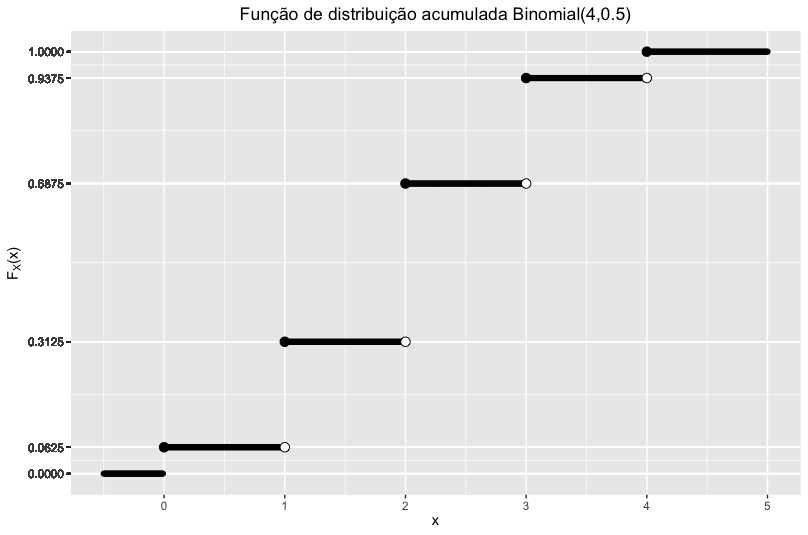
\includegraphics[width=\textwidth]{C2Q1.png}
\section{Questão 2}

\section{Questão 3}
\section{Questão 4}
\section{Questão 5}
\section{Questão 6}
\section{Questão 7}
\section{Questão 8}
\section{Questão 9}
$$ 
f(x)=\begin{cases}
\frac{1}{(1+x)^2}, x>0\\
0 \ \ \  \ \ \ ,x<0
\end{cases}
$$

$$Y=max(X,c)=\begin{cases}
X, X> c\\
c, X\le c
\end{cases} $$

$$P(X=Y\le y,X>c) + P(Y=c,Y\le y, X\le c) $$
$$F_Y(x)=\begin{cases}
0, x<0\\
\frac{x}{(1+x)},x>c\\


\end{cases}  $$
\section{Questão 10}

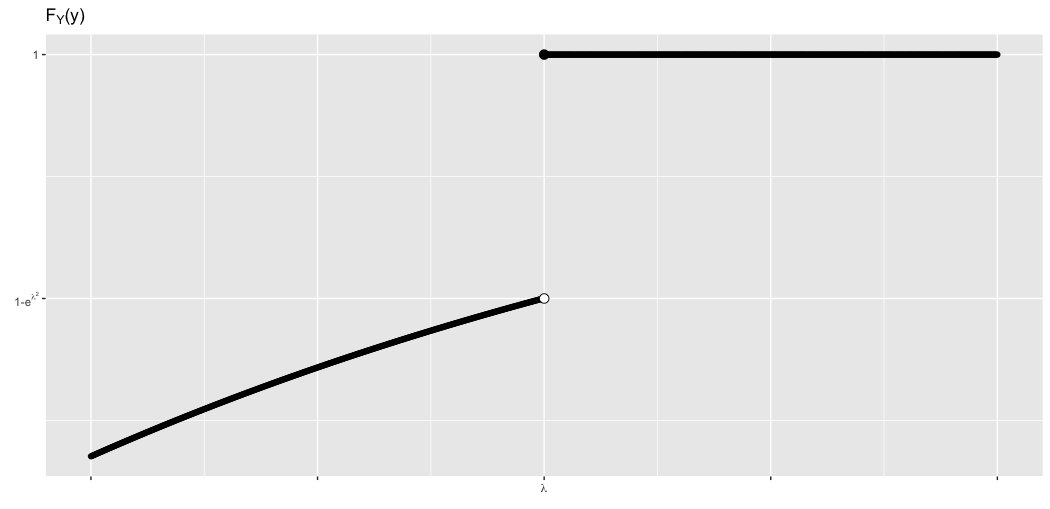
\includegraphics[width=\textwidth]{C2Q10.png}'

$$Y=\begin{cases}
1 , X>1\\
X, X<1\\
\end{cases} $$
se y<0 então FY = 0 pois X só assume valores no intervalo [0,1]\\
Se y< X , então $F_Y(x^-)$ = $F_z: Z\sim U[0,x]$\\
se  x<y<1\\
$F_Y$\\
$F_y = \begin{cases}
0, y<0\\
x/2 , y<x<1\\
1, x>1

\end{cases} $
$$
Y=\begin{cases}
X, X>2\\
2. X<2
\end{cases}
$$
$y<0, F_y=0 $\\
 $0<y<2 $ ,Fy = 0\\
 y>=2 , FY = 1- exp(-2y)
 $$F_y= \begin{cases}
 0, y<0\\
 1-e^{-2y} , y\ge 2
 \end{cases} 
 $$
 $$F_{ac} = \begin{cases}
0, y< 2\\
 e^{-4}-e^{-2y},y\ge2
 \end{cases} $$
 
 $$ F_d =\begin{cases}
 0, y<2\\
1-e^{-4}, y\ge 2
 
 \end{cases}$$ 
 



	
	
\end{document}